\documentclass [letterpaper,12pt]{report}

\usepackage {graphicx}
\usepackage {times}
\usepackage {fancyhdr}
\usepackage[hmargin=1in,vmargin=1.25in]{geometry}
\usepackage {mathptmx, amsfonts}
\usepackage [chapter]{algorithm}
\usepackage [noend]{algorithmic}
\usepackage {url}
\usepackage[T1]{fontenc}
\usepackage {verbatim}
\usepackage {microtype}
\usepackage[labelfont=bf]{caption}
\pagestyle {fancy}
\graphicspath{{./images/}}
\begin {document}

% Setup header and footer
\fancyhf{} % clear all fields
\fancyfoot[R]{Open Motion Planning Library : A Primer $\|$ \thepage}
\renewcommand{\chaptermark}[1]{\markboth{\chaptername\ \thechapter.\ #1}{}}
\fancyhead[C]{\leftmark}

% Inserting title page
\begin{titlepage}

\begin{center}


% Upper part of the page

\begin {figure}
\centering

\includegraphics[width=2.5in]{RiceLogo}
\end{figure}
\vspace {0.25in}
\rule{\linewidth}{0.1mm}
\vspace {0.25in}

% Title
{ \huge \bfseries Open Motion Planning Library:\\ A Primer}
\\ [0.50in]
{\Large Kavraki Lab\\
Rice University
}
\\ [0.1in]
{\tt ompl.kavrakilab.org}

%\HRule \\[1.5cm]

\vfill

{\large \today}

\end{center}

\end{titlepage}


% Generate Table of Contents with roman numeral page numbering
\newpage
\pagenumbering{roman}
\tableofcontents

% Ensure the rest of the document has arabic numerals
\newpage
\pagenumbering{arabic}

\chapter{Introduction}

This document explains how the Open Motion Planning Library (OMPL) implements
the basic primitives of sampling-based motion planning, what planners are
already available in OMPL, and how to use the library to build new planners.
This primer is segmented into the following sections: An introduction to
sampling-based motion planning, a guide to setup OMPL for solving motion
planning queries using OMPL.app, a description of the motion planning
primitives in OMPL to develop your own planner, and an explanation of
some advanced OMPL topics.

At the end of this document, users should be able to use OMPL.app to solve
motion planning queries in 2D and 3D workspaces, and utilize the OMPL framework
to develop their own algorithms for state sampling, collision checking, nearest
neighbor searching, and other components of sampling-based methods to build
a new planner.


\section {Prerequisites for Using OMPL}
This primer assumes that users are familiar with C++ programming and compiling
code in a Unix environment.  Additionally, users should have basic knowledge of
sampling-based motion planning.  OMPL and OMPL.app should also be installed.
For information regarding the installation process, please see
{\tt ompl.kavrakilab.org}.



\chapter{Introduction to Sampling-based Motion Planning}
\label{chp:motionplanning}

To put OMPL in context, a short introduction to the principles of
sampling-based motion planning is first given.  Robotic motion planning seeks
to find a solution to the problem of ``Go from the start to the goal while
respecting all of the robot's constraints."  From a computational sense,
however, such an inquiry can be very difficult due to the potential for a large
number of degrees of freedom for the robot.  For simplicity, consider the
classical motion planning problem known as the piano mover's problem.  In this
formulation, there exists a rigid object in 3D (the piano), as well as a set of
known obstacles.  The goal of the piano mover's problem is to find the shortest,
collision-free path for the piano that begins at its starting position and
ending at a prescribed goal configuration.  Computing the exact solution to
this problem is very difficult.  In this setup, the piano has six degrees of
freedom: three for movement in the coordinate planes ($x$,$y$,$z$), and three
more to represent rotation along the axes of these coordinate planes (roll,
pitch, yaw).  To solve the piano mover's problem we must compute a set of
continuous changes in all six of these values in order to navigate the piano
from its starting configuration to the goal configuration while avoiding
obstacles in the environment.  It has been shown that finding a solution for
the piano mover's problem is {\tt PSPACE}-hard, indicating computational
intractability in the degrees of freedom of the robot \cite{Latombe:1991,
Choset:2005, LaValle:2006}.

\section {Historical Notes}
OMPL specializes in sampling-based motion planning, which is presented in
section~\ref {sect:samplingbasedplanning}.  To put sampling-based methods
in context, a brief historical overview to the methods that have been proposed
for motion planning is presented.  Most of these methods were developed before
sampling-based planning, and are still applicable in many applications.

\paragraph {Cell Decomposition}
In some instances, it is possible to partition the workspace into discrete
cells corresponding to the obstacle free portion of the environment.  This
decomposition can then be modeled as a graph (roadmap), where the vertices
represent the individual cells and edges indicate adjacency among the cells.
Utilizing this graph, the problem becomes a classical search from the cell with
the starting position to the cell containing the goal position.  Such a
formulation works well in ``controllable'' systems (e.g., an omni-directional base).
However, when using a robot with complex dynamics it may not be possible for the
system to move to an adjacent cell in the decomposition given the constraints
of motion.  Moreover, the movement of a robot is typically performed in its
state space, which may be of much higher dimension than the workspace.
Decomposing the robot's state space in the same manner is possible, but
practically such computation is infeasible.

\paragraph {Control-based Methods}
Control-based methods attempt to model the equations of motion of the system
and apply ideas from control theory in order to navigate a system along a
specified trajectory.  These approaches operate in the continuous space, and
typically employ a feedback loop in order to effectively maneuver the system
with minimal error.  Using a control-based approach to navigate a robot is
very fast and can be done in an online manner, which is necessary in many
applications.  Computing a desirable and feasible trajectory can be very
difficult, however, in systems with complex dynamics and/or cluttered
environments, which heavily restrict the valid motions.

\paragraph {Potential Fields}
Conceptually, potential fields are a simple and intuitive idea.  The classical
potential field involves computing a vector at each point in the workspace by
calculating the sum of an attractive force emanating from the goal, and a
repulsive force from all of the obstacles. The system can then navigate
using gradient descent to follow the potentials to the goal. Similar to
control-based methods, potential fields can be applied to a wide variety of
systems and can operate in real-time.  Navigating a system using a potential
field, however, can fail due to local minima in the field itself, which stem
from the heuristic combination of the forces in the workspace.  Ideally the
field would be constructed in the state space of the system, but this is
equivalent to solving the original problem.  Some approaches consider a {\it
navigation function} where the potential field is guaranteed to have a single
minimum, but computing such a function is non-trivial in some environments,
especially cluttered workspaces.

\paragraph {Randomized Planning}
Randomization in otherwise deterministic planners has shown to be very
effective.  In potential fields, for example, Brownian motions in which a random
action is applied for a specific amount of time have been shown to be highly
effective in guiding a system out of a local minima.  Using randomization is
also possible for planning the motions of high-dimensional or non-holonomic
systems, where the previous deterministic do not perform well.  Sampling-based
techniques are a subset of randomized planning algorithms that are particularly
effective for high degree of freedom or systems with complex dynamics.

\section {Sampling-based Motion Planning}
\label {sect:samplingbasedplanning}
Sampling-based motion planning is a powerful concept that employs random
sampling of the state space of the robot in order to quickly and
effectively answer planning queries, especially for systems with non-holonomic
constraints or those with many degrees of freedom.  Traditional approaches to
solving these particular problems may take a very long time due to motion
constraints or the size of the state space.  Sampling arises out of the need to
quickly cover a potentially large and complex state space to connect a start
and goal configuration along a feasible and valid path.

The need to reason over the entire continuous state space causes traditional
approaches to breakdown in high-dimensional spaces.  In contrast, sampling-based
motion planning reasons over a finite set of configurations in the state space.
The sampling process itself computes a (generally uniform) set of random robot
configurations, and connects these samples via collision free paths that respect
the motion constraints of the robot to answer the query.  Because the continuous
state space is not explicitly reasoned over, sampling-based methods provide {\it
probabilistic completeness}.  This indicates that the planner is not guaranteed
to find a solution, but the probability of finding a solution converges to one
as the number of samples reasoned over increases to infinity.  This should not
be confused with algorithmic completeness; sampling-based approaches cannot
recognize a problem with no solution.

\subsection {Problem Statement and Definitions}
This section will present the problem to be solved by the motion query using
a sampling-based method, and define some useful terminology that will be used
throughout the remainder of the primer.

\begin{description}
\item[Workspace:] The physical space that the robot operates in.  It is
assumed that the boundary of the workspace represents an obstacle for the robot.
\item[State space:] The parameter space for the robot.  This space
represents all possible configurations of the robot in the workspace.  A single
point in the state space is a {\it state}.
\item[Free state space:] A subset of the state space in which each state
corresponds to an obstacle free configuration of the robot embedded in the
workspace.
\item[Path:] A continuous mapping of states in the state space.  The path
collision free if each element of the path is an element of the free state
space.
\end{description}

From these definitions, the goal of a sampling-based motion planning query can
be formalized as the task of finding a collision path in the state space of the
robot from a distinct start state to a specific goal state, utilizing a path
composed of random configurations connected by collision free paths.

The remainder of this section will discuss two types of sampling-based planners,
from which many of the state of the art techniques can be derived from.

\subsection {Probabilistic Roadmap}
The probabilistic roadmap ({\tt PRM}) is among the first sampling-based motion
planners \cite {Kavraki:1996}.  This approach utilizes random sampling of
the state space to build a roadmap of the free state space.  This roadmap is
analogous to a street map of a city.  To illustrate the fundamentals of the
{\tt PRM}, a simple example of a 2D workspace and freely moving point robot will
 be used.

\begin {figure}[h]
\centering
{
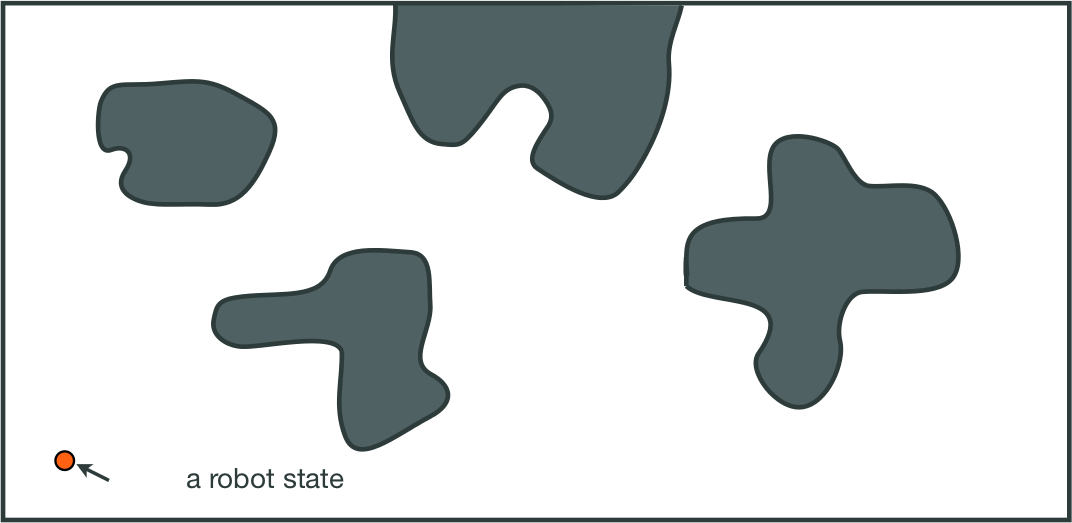
\includegraphics [width=3.75in]{state}
\caption {The 2D workspace and a single state for the point robot.}
\label {fig:prm:state}}
\end {figure}

Consider the workspace in figure \ref{fig:prm:state}.  This image shows a
bounded workspace for the point robot in which the shaded regions are obstacles.
One particular state for the robot is highlighted.  The {\tt PRM} works by
uniformly sampling the free state space and making connections between the
samples to form a roadmap of the free state space.  The roadmap can be stored
efficiently as a graph data structure where the random samples compose the
vertices, as in figure \ref{fig:prm:samples}.  It should be noted that the free
state space is almost never explicitly known in sampling-based methods. Each
sample that is generated is checked for collision, and only collision free
samples are retained. Additionally, there are many different ways to sample the
free state space, and changing the sampling strategy is beneficial in many
planning instances.

\begin {figure} [h]
\centering
{
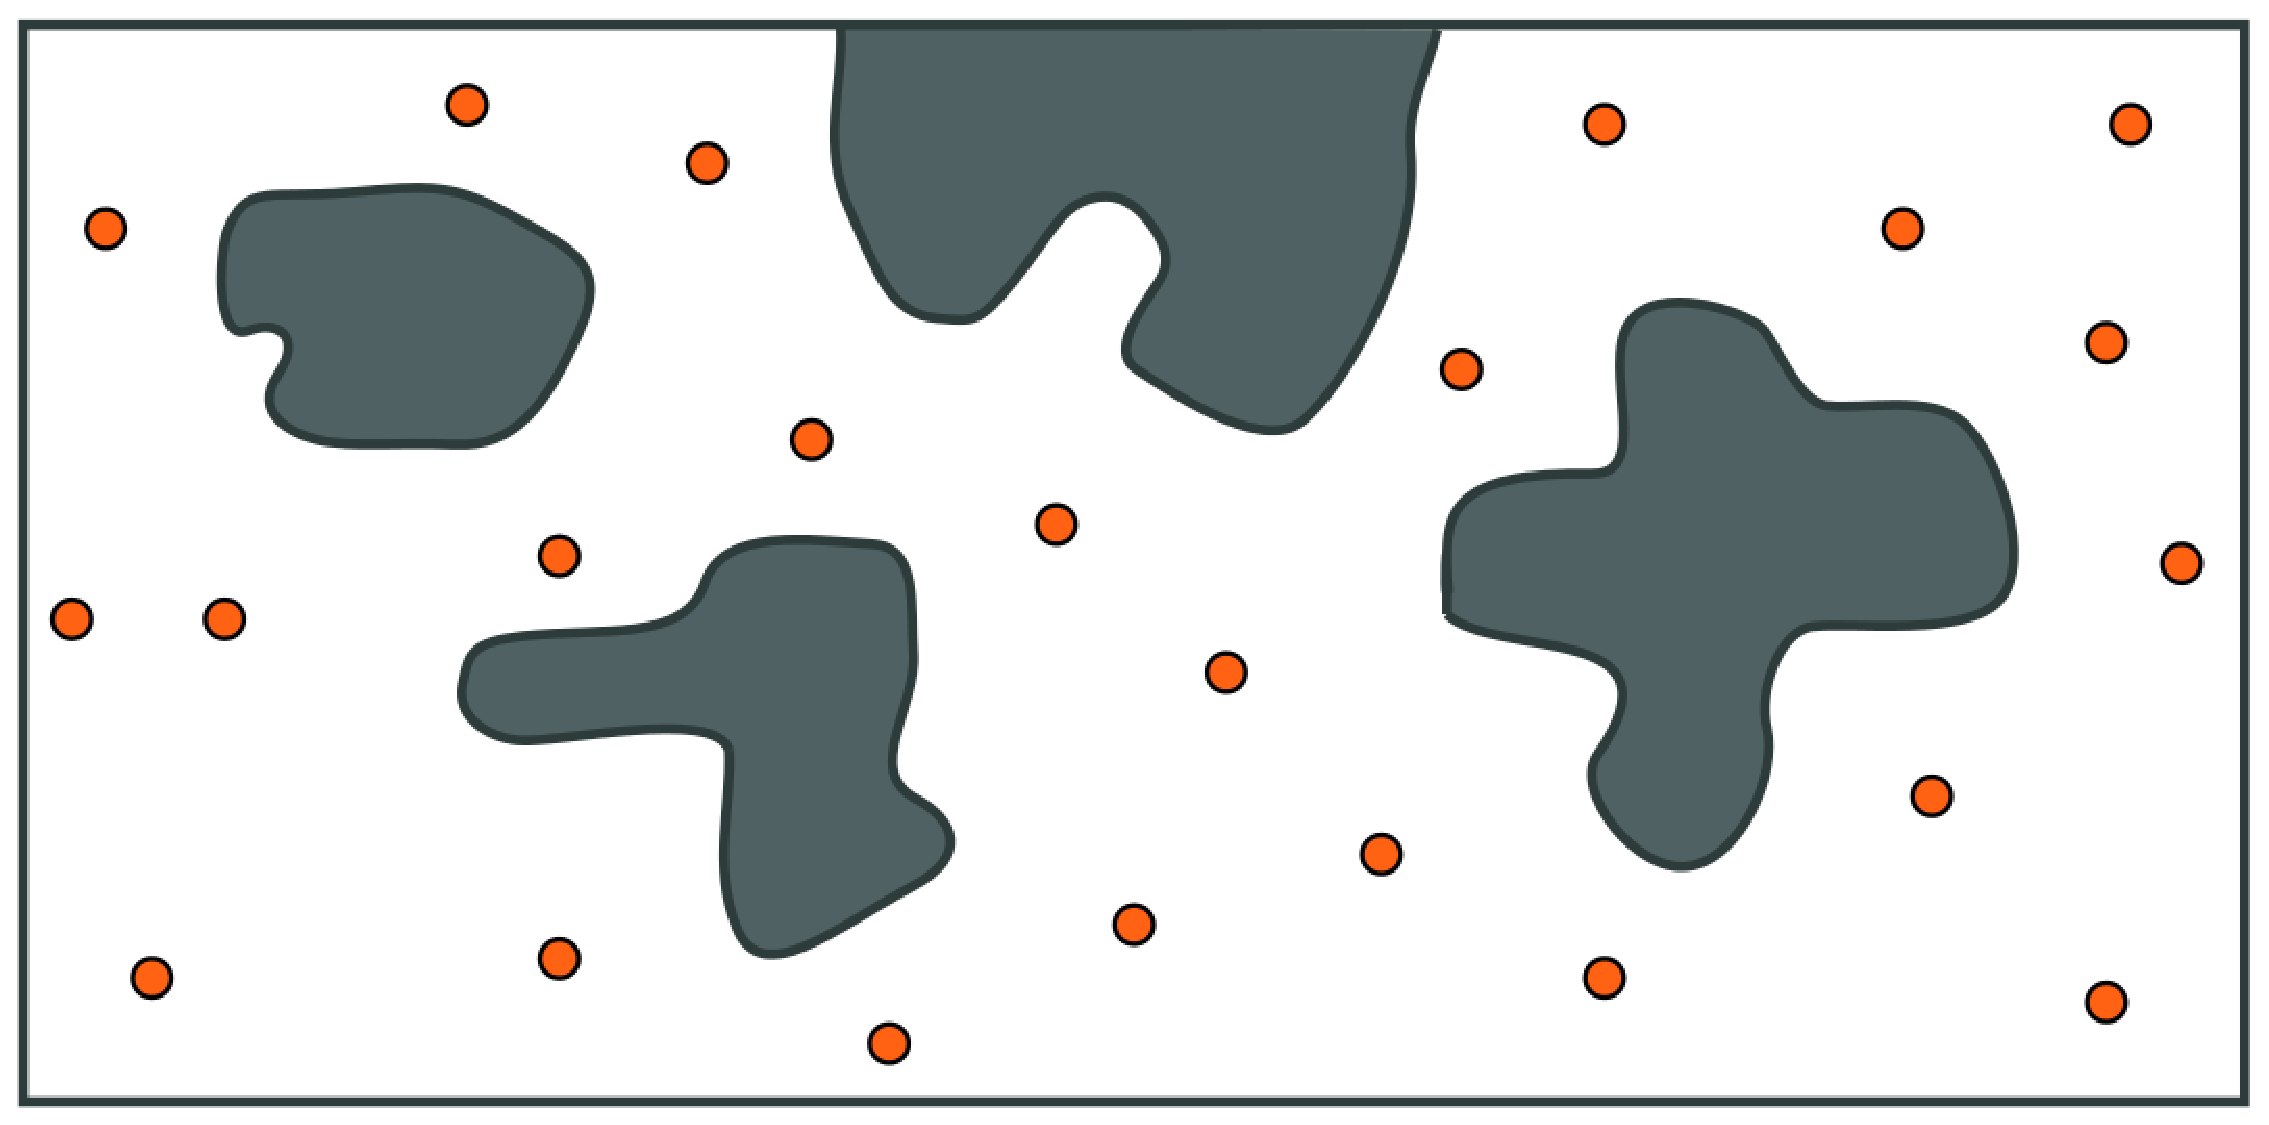
\includegraphics [width=3.75in]{samples}
\caption {One possible set of uniform random samples of the free state space}
\label {fig:prm:samples}
}
\end {figure}

Once the desired number of free samples have been found, the roadmap itself can
be constructed by connecting the random samples to form the edges.  The
canonical {\tt PRM} attempts to connect each sample to the $k$ samples nearest
to it by using a local planner that is tasked with finding short collision free
paths. The local planner finds this path by interpolating the motion of the
robot between the two samples, checking for collisions at some prescribed
resolution.  If no configuration of the robot between the samples collides with
an obstacle, then an edge is inserted to the roadmap.  Figure \ref
{fig:prm:localplanner} shows a complete probabilistic roadmap in the 2D
workspace example.

\begin {figure}[h]
\centering
{
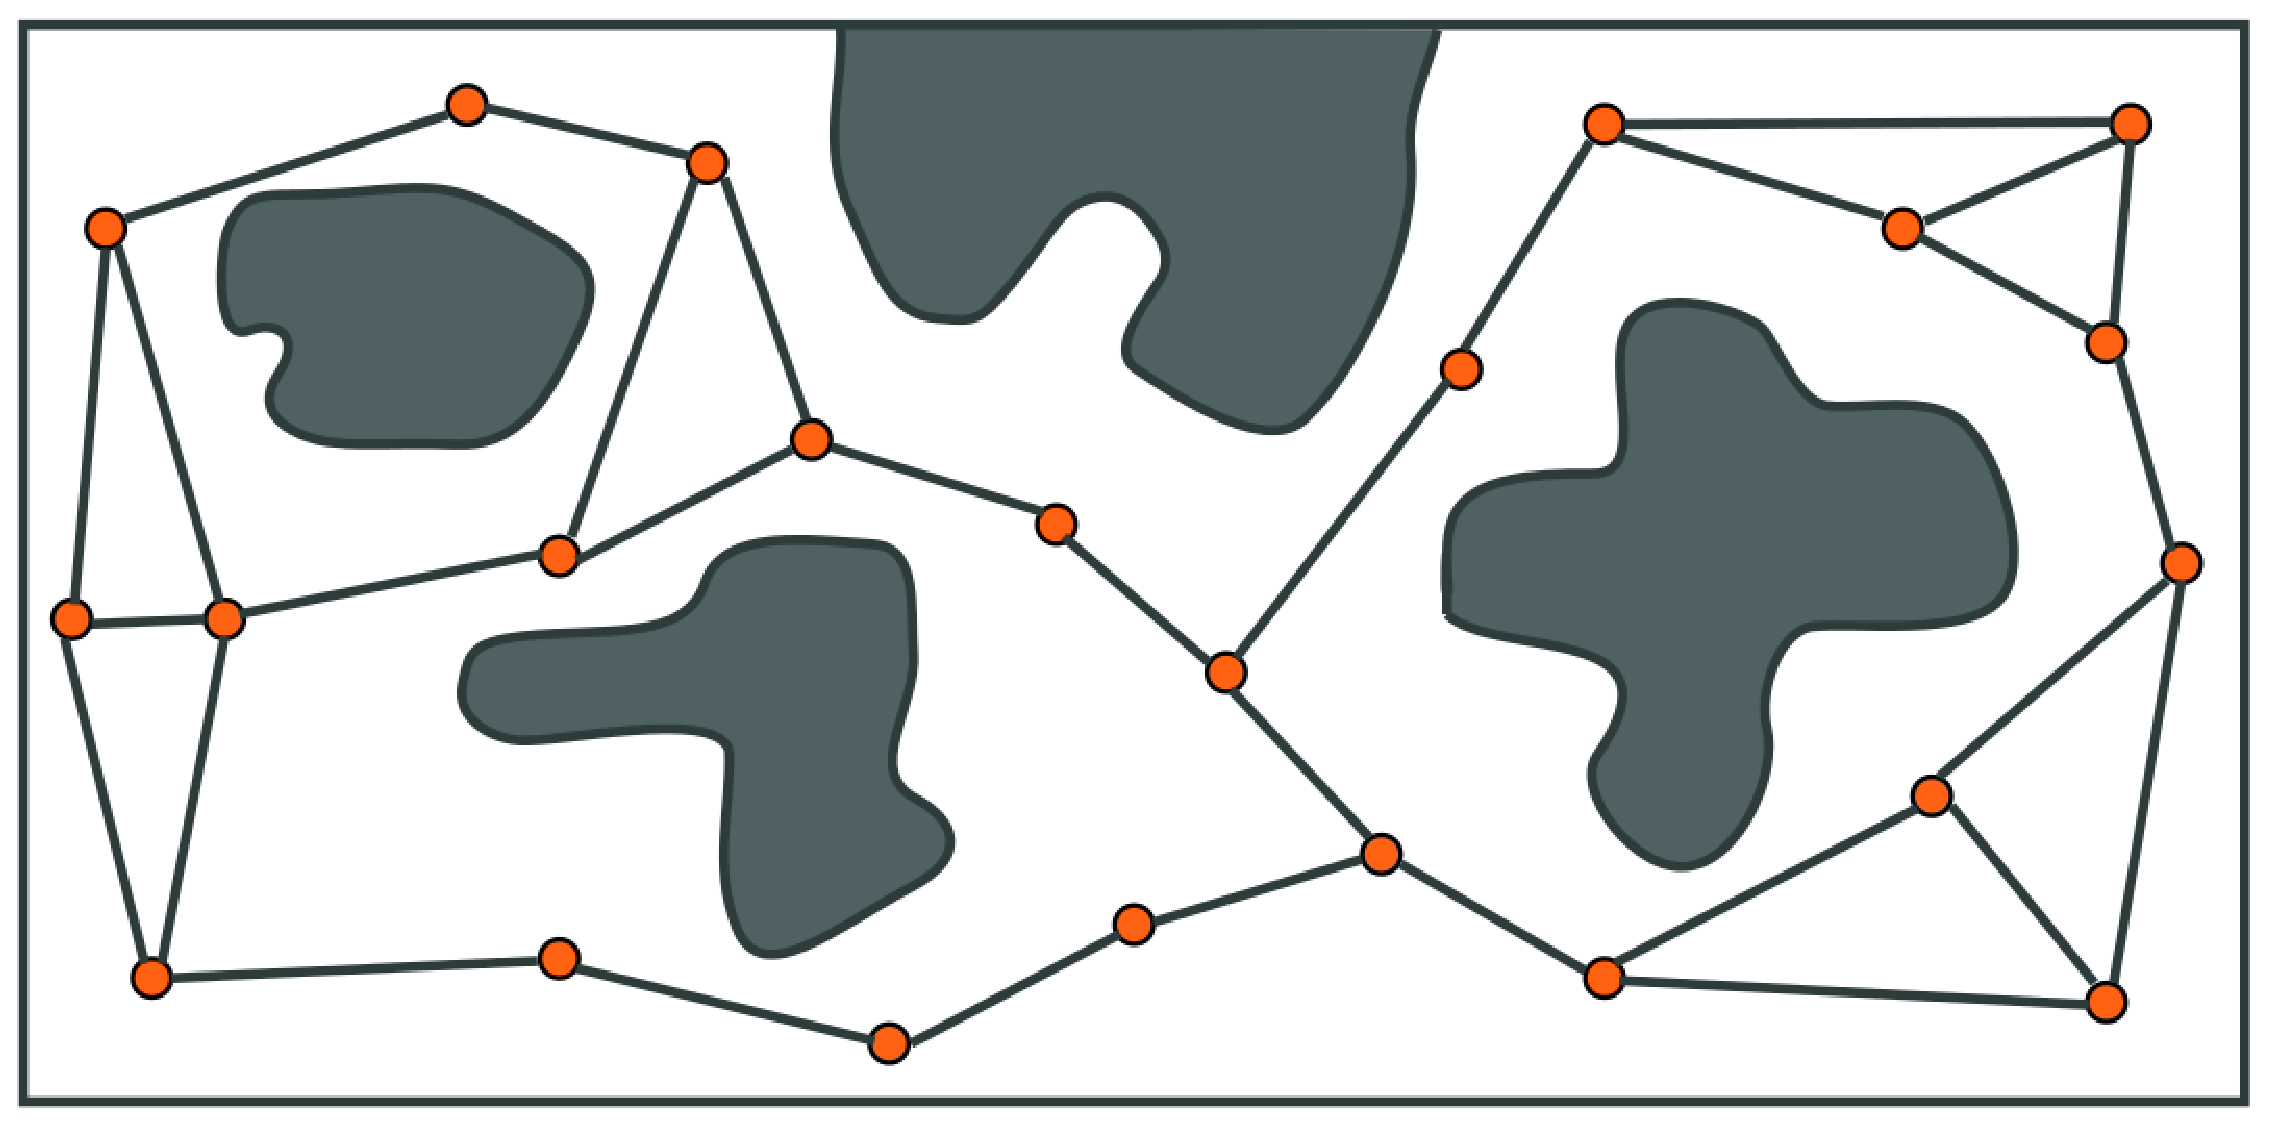
\includegraphics [width=3.75in]{localplanner}
\caption {Using a local planner, the {\tt PRM} is formed by connecting samples
that are close to one another using a straight path in the free state space.}
\label {fig:prm:localplanner}
}
\end {figure}

Once the roadmap is complete, it can be used to answer motion planning queries
by connecting the start and goal states to the roadmap using the local planner,
and performing a graph search to find the shortest path in the roadmap.  This
is seen in figure \ref {fig:prm:query}.

\begin {figure}[h]
\centering
{
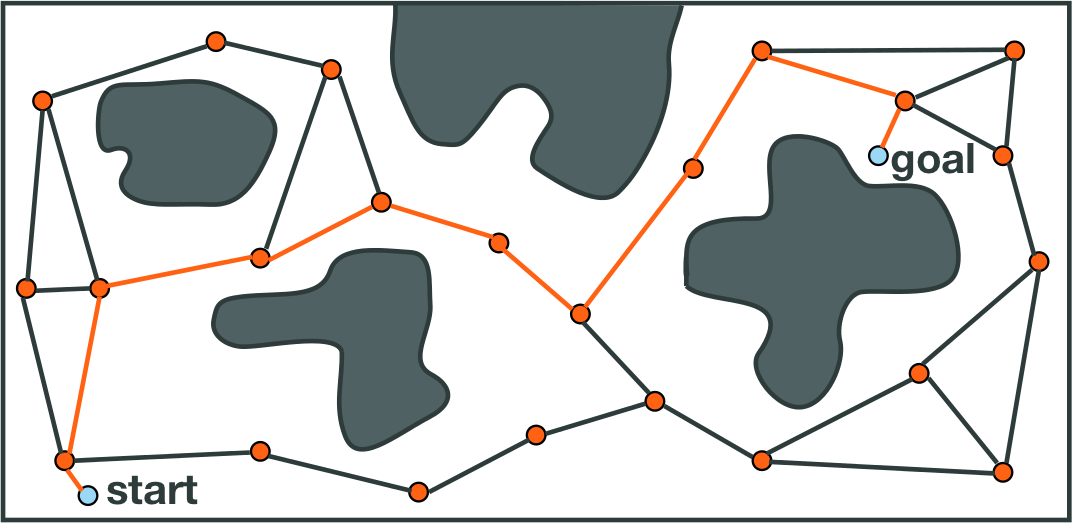
\includegraphics [width=3.75in]{query}
\caption {An example of a motion planning query on a {\tt PRM}.  The start and
the goal are connected to the roadmap, and the shortest path in the graph is
found.}
\label {fig:prm:query}
}
\end {figure}

\subsection {Tree-based Planners}
There exist many types of sampling-based planners that create tree structures
of the free state space.  The trees generated by these methods are analogous to
the probabilistic roadmap, except that the structure contains no cycles.  Due to
the wide variety of tree-based planners (e.g. {\tt RRT}\cite {LaValle:2001},
{\tt EST}\cite{Hsu:1999}, {\tt SBL}\cite{Sanchez:2003},
{\tt KPIECE}\cite{Sucan:2011}), one specific type will not be discussed in detail here.  However,
a general framework will be described.  These methods begin by rooting a tree at
the configuration where the robot begins.  With the first node of the tree intact,
random sampling of the free space then occurs.  The planner employs an
expansion heuristic, which typically gives the method its name, from which the
sample is connected to the tree along a collision free path.  Figure
\ref{fig:tree:start} shows an example in the 2D workspace scenario where the first
few valid samples are connected to the tree.

\begin {figure}[h]
\centering
{
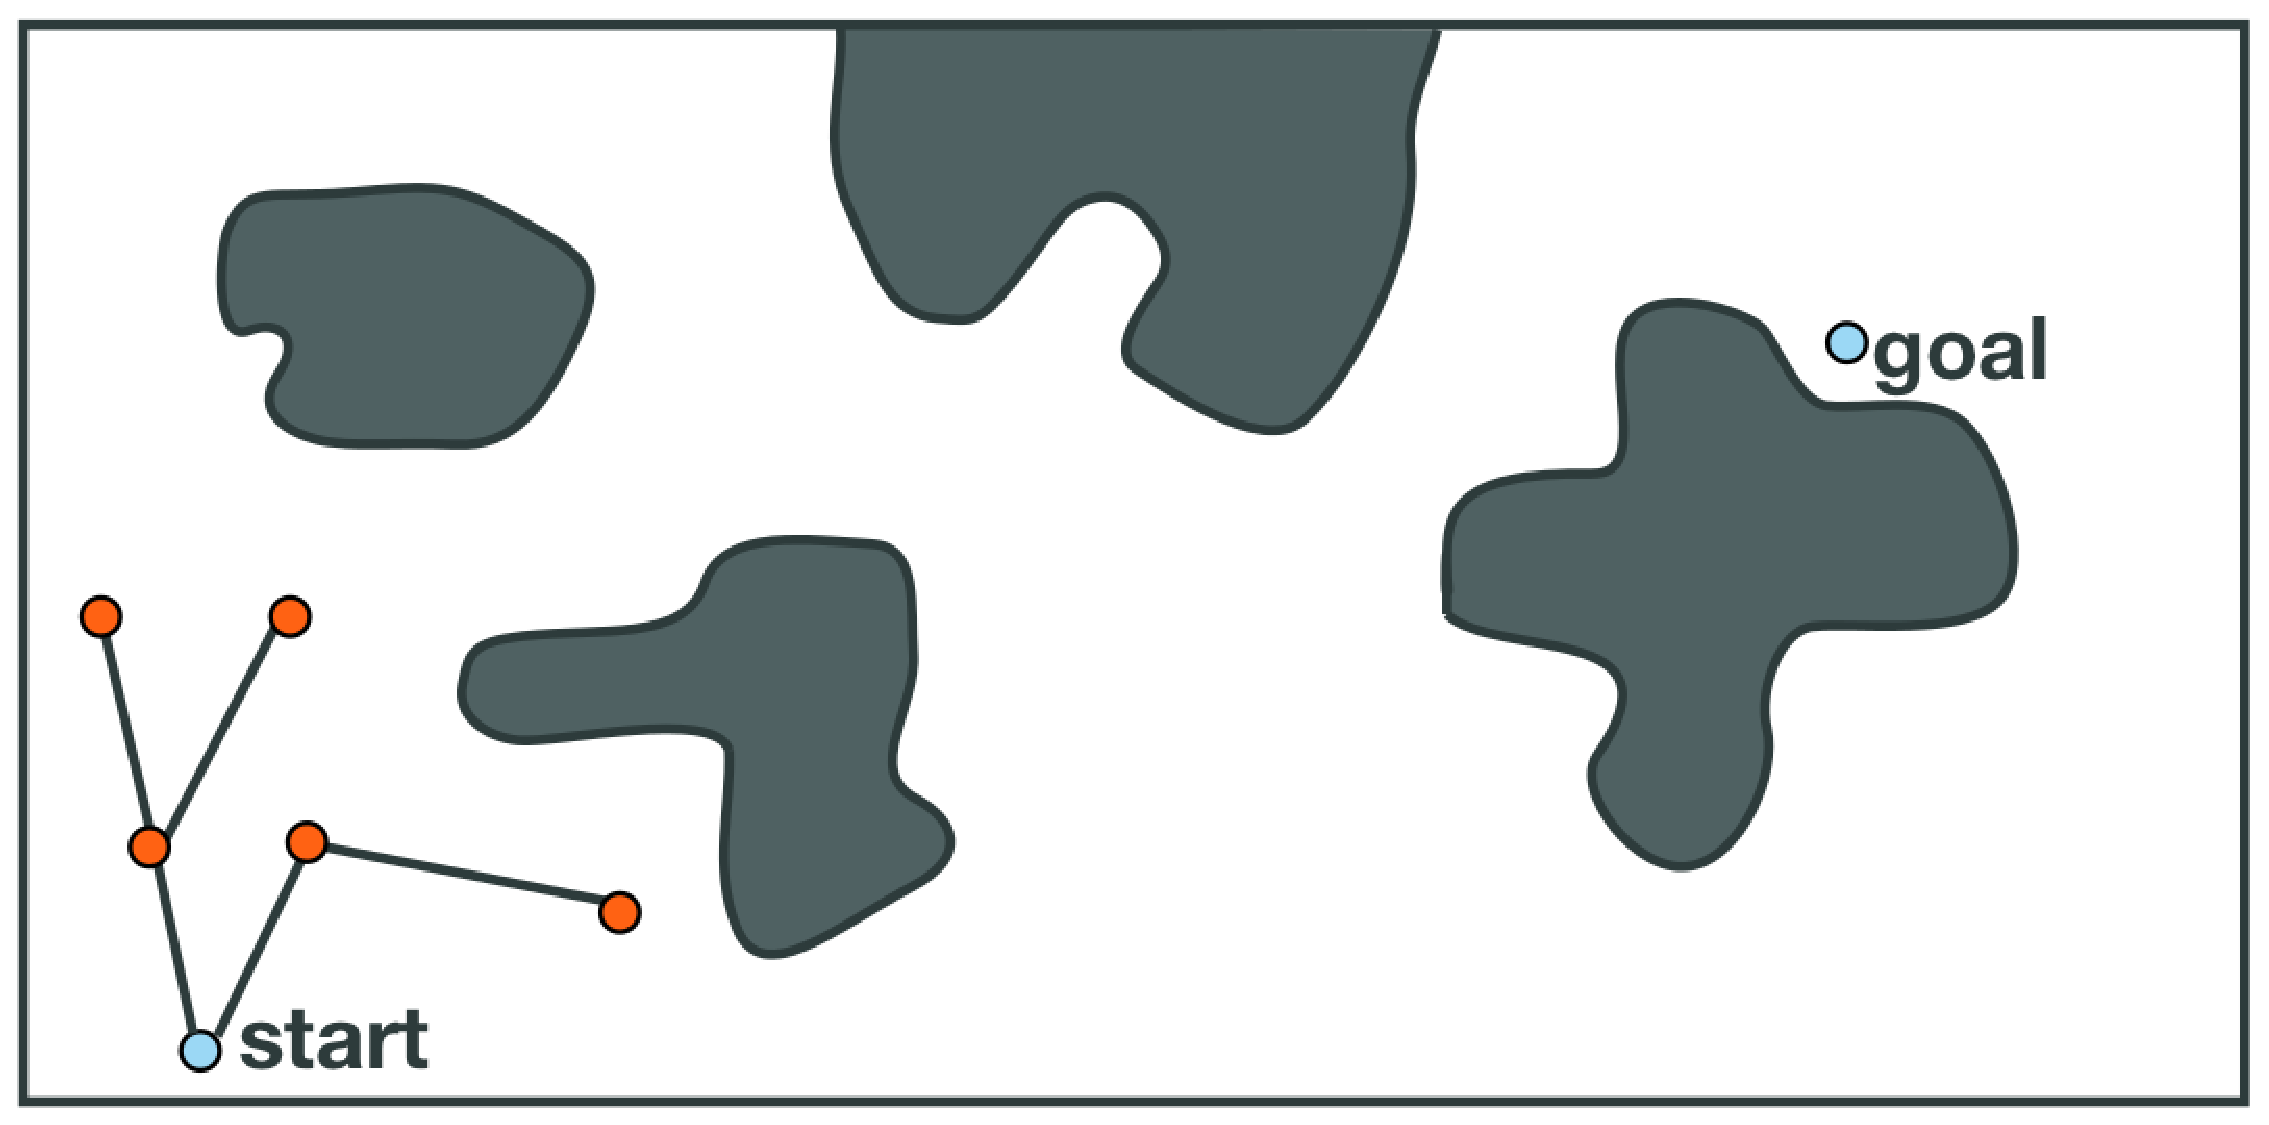
\includegraphics [width=3.75in]{tree-start}
\caption {The sampling observed after the first few samples have been connected.
Random samples are connected to the tree using an expansion heuristic.}
\label {fig:tree:start}
}
\end {figure}

Since it is highly improbable that the sampling process will ever sample the
goal state exactly, the methods often bias the expansion of the tree toward
the goal state.  If it is possible to connect the goal to the existing
tree, then the search is complete; a path through the free state space has been
found from the start to the goal.  Figure \ref{fig:tree:badgoal} shows a case
where the goal cannot be connected to the tree, and Figure \ref{fig:tree:goal}
shows the case where the goal is connected, terminating the search.

\begin {figure}[h]
\centering
{
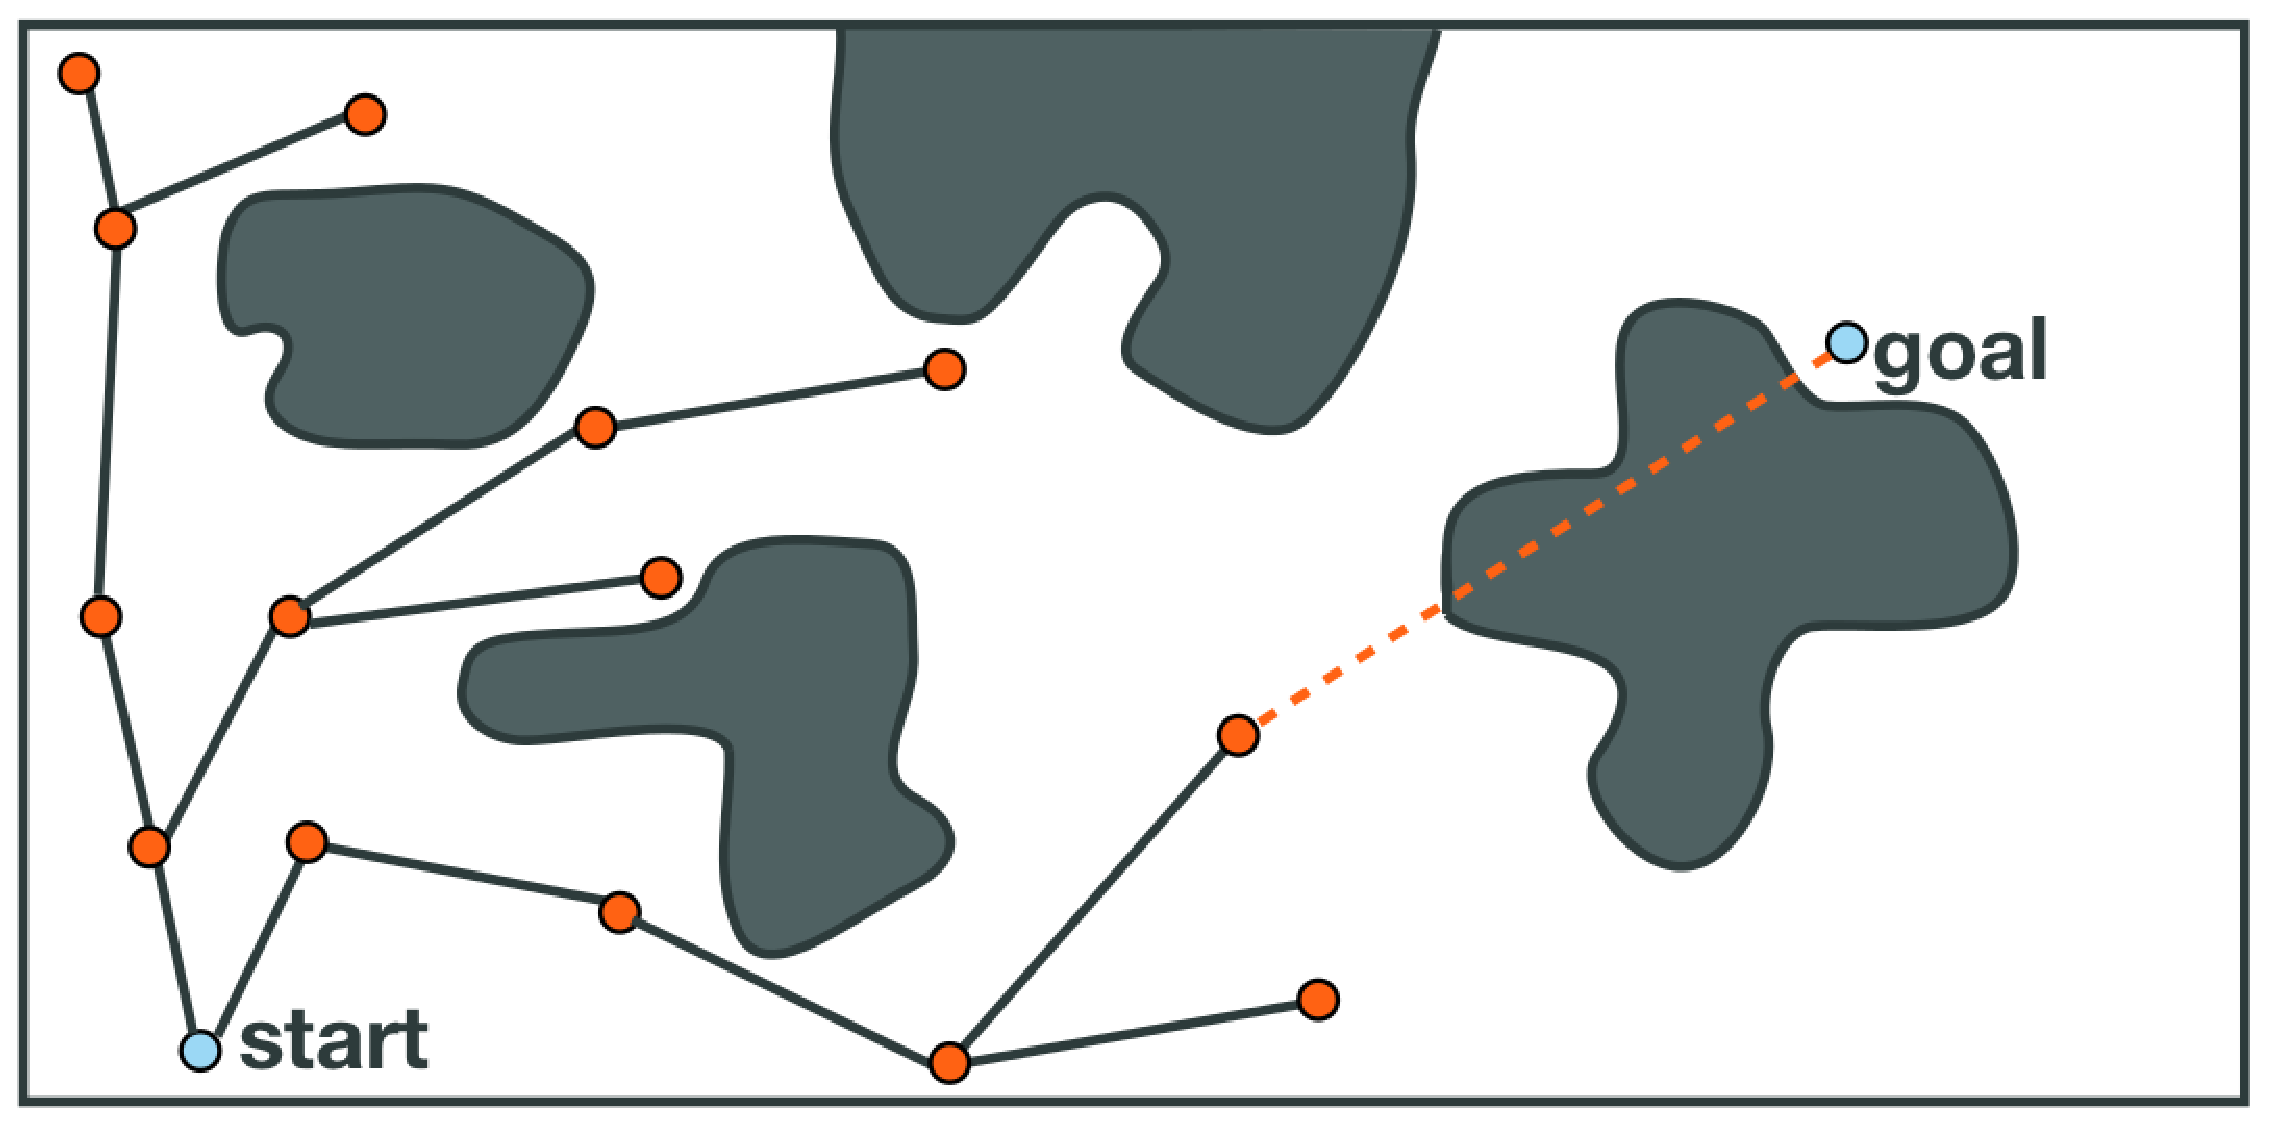
\includegraphics [width=3.75in]{tree_badgoal}
\caption {Scenario where the goal is selected during the sampling process, but
cannot be connected to the tree.  The closest node in the tree is obscured by
an obstacle.}
\label {fig:tree:badgoal}
}
\end {figure}

It is important to highlight the difference between the roadmap-based planners
and the tree-based planners. The tree-based techniques are only good for
single-query planning.  These trees do not normally cover the free space in the
same manner that a roadmap would.  However, when planning with differential
constraints, it isn't easy to encode control information into an undirected edge.
Controls are usually directed commands, and require a specific pre-condition in
order for a particular control to be valid.  Tree-based methods, on the other
hand, excel at planning with complex dynamics because of the directed, acyclic
nature of the underlying data structure.  Control information can be encoded
for each edge of the tree, with the vertices of the tree satisfying the
prerequisites for the valid controls.

\begin {figure}[h]
\centering
{
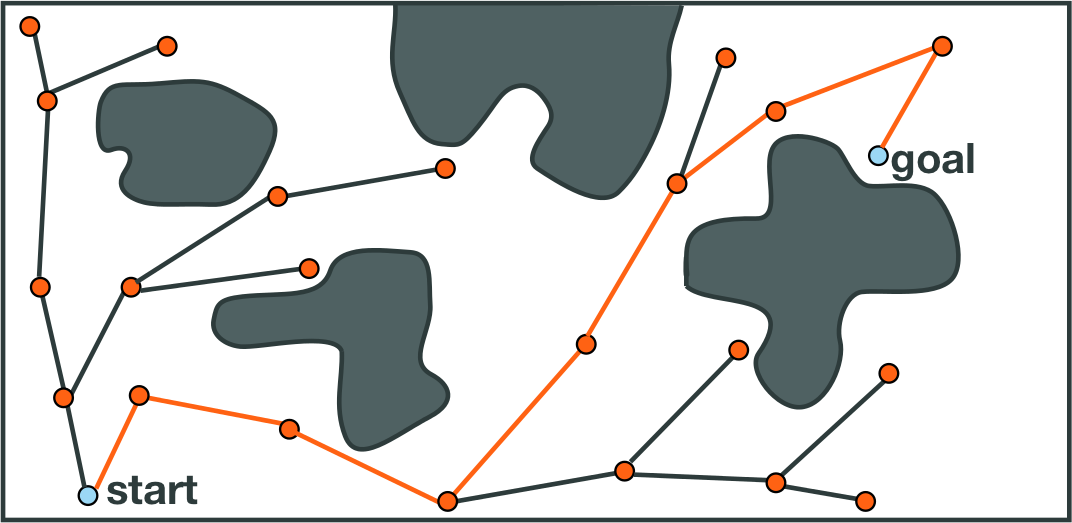
\includegraphics [width=3.75in]{tree_goal}
\caption {Scenario where the goal is selected during the sampling process, and
is connected to the tree, ending the search.}
\label {fig:tree:goal}
}
\end {figure}

Finally, it should be noted that many sampling-based approaches require a much
smaller memory footprint than other motion planners.  The compactness of these
planners stems from the sampling process itself, as well as the fact that no
explicit representation of the state space is needed in order to solve the
problem.  Storage and search of the underlying data structure (e.g. graph, tree)
should be efficient to fully maximize the quality of these methods.

%\clearpage
\subsection {Primitives of Sampling-based Planning}
Sampling-based planning is a very powerful tool for planning in high dimensional
spaces or for system with complex dynamics.  There exists many kinds of
sampling-based motion planners, with many commonalities, but the method in which you
sample the state space is key to computing a solution.

Collision checking is a very important part of sampling-based planning.  It is
used not only in the local planner when attempting to find collision free paths
between samples, but also during the sampling process itself.  In a complex or
high-dimensional system it may not be easy to explicitly represent the free
state space, but in sampling-based methods it isn't necessary to create this
space.  It is the job of the collision checker to accept a configuration of the
robot and quickly determine whether or not this state is in collision.

Nearest neighbor searching is another cornerstone of sampling-based methods.
It is from the ability of determining whether two states of the robot are close
that many of the common approaches are able to effectively find paths through a
high dimensional space.  Distances, however, are not easy to compute in
non-euclidean spaces where many of the interesting problems reside.  Kd-trees
offer one way to perform this search, but the optimal connection strategy for
samples remains elusive.

The core OMPL library cleanly implements all of these primitives of
sampling-based motion planning.  Chapter \ref{chp:ompl.app} shows how the
planners bundled with OMPL can be used to directly solve motion planning
queries, and chapter \ref{chp:ompl} details how these primitives map to concepts
within the open motion planning library.



\chapter{Getting Started with OMPL.app}
\label {chp:ompl.app}

OMPL.app provides a graphical front-end to the core OMPL library, and allows
a user to see many of the ideas from sampling-based motion planning in action.
The GUI is written using Python and PyQt.  OMPL.app comes bundled with
the core OMPL library, and can be found at {\tt ompl.kavrakilab.org}.

By using OMPL.app, introductory users to OMPL can get a sense of the current
capabilities of the library and sampling-based motion planning.  Currently,
users can use geometric motion planning for rigid bodies in 2D and 3D,
control a variety of simplified kinodynamic systems (e.g., unicycle, blimp,
or car), and even a dynamic car using the Open Dynamics Engine.  OMPL.app
also demonstrates one possible way of representing the geometry of the robot
and how to provide collision checking to the core library using a particular
geometric representation.

\section {Using OMPL.app}

To launch OMPL.app, execute the {\tt ompl\_app.py} python script, which is found
in the {\tt omplapp/ gui} directory.  When the GUI is loaded, a window will be
presented as in Figure \ref{fig:omplapp:start}.

\begin {figure}[h]
\centering
{
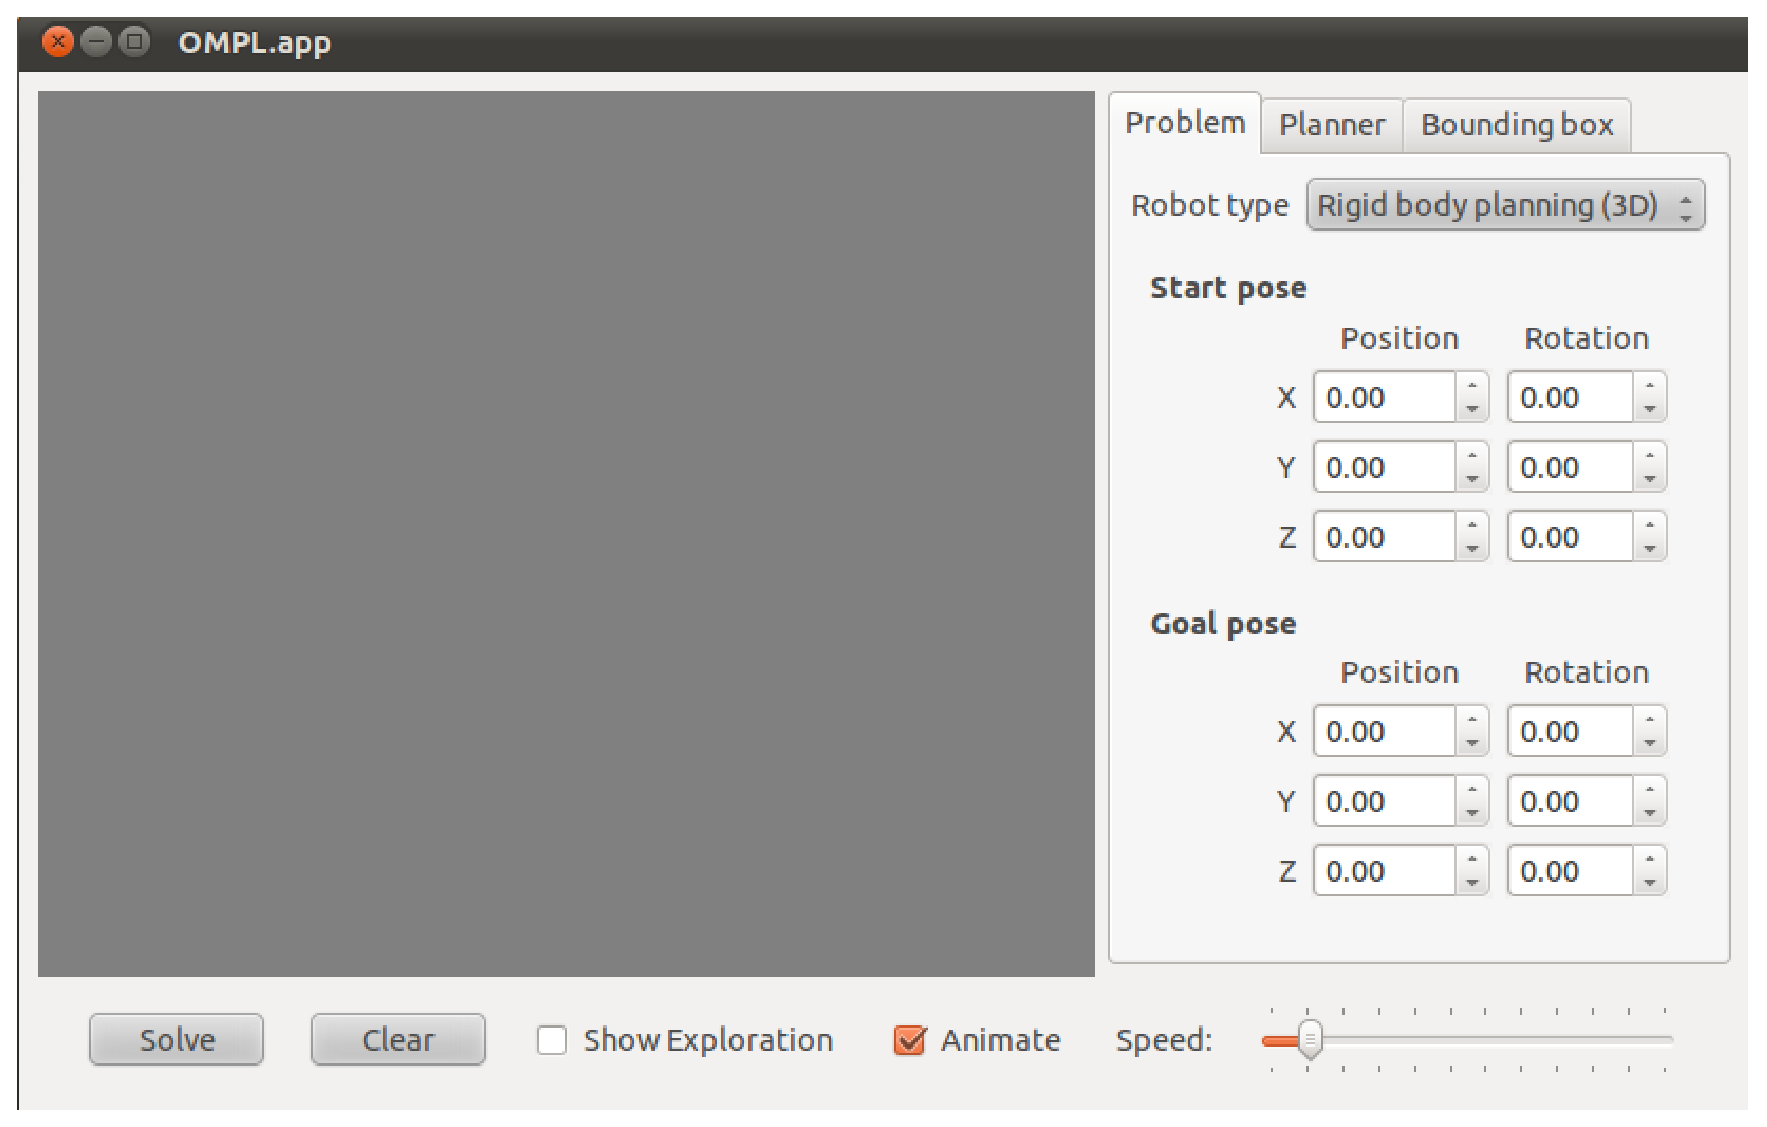
\includegraphics [width=3.5in]{omplapp_start}
\caption {OMPL.app at startup}
\label {fig:omplapp:start}
}
\end {figure}


OMPL.app requires us to do three things to solve a motion planning query: setup the
workspace and the robot, select a planner to use, and bound the environment.
These three items correspond to the tabs located in the upper right portion of
the window.

\subsection {Selecting a Robot and an Environment}
First, a robot type must be selected.  The traditional ``piano mover's'' problem
is a rigid body planning in 3D instance, so select ``Rigid body planning (3D)''.
Next, the environment and the robot itself must be loaded.  OMPL.app comes
packaged with a number of mesh models for 2D and 3D environments and robots.
Go to the {\it File} menu at the top of the window and select
{\it Open Environment}.  This presents a dialog screen to open a file.  Navigate
to the {\tt omplapp/resources/3D} directory and select the {\tt Easy\_env.dae}
mesh to load.  Then select {\it Open Robot} from the file menu and open
{\tt Easy\_robot.dae} from the same directory.  When the meshes are loaded, you
will see an environment consisting of a wall partitioning the space into two
parts with a small opening in the center (Figure \ref{fig:omplapp:easy}).
Rotate the view using the mouse to see both sides of the partitioned space and
the ``L'' shaped robot inside the opening of the wall.

\begin {figure}[h]
\centering
{
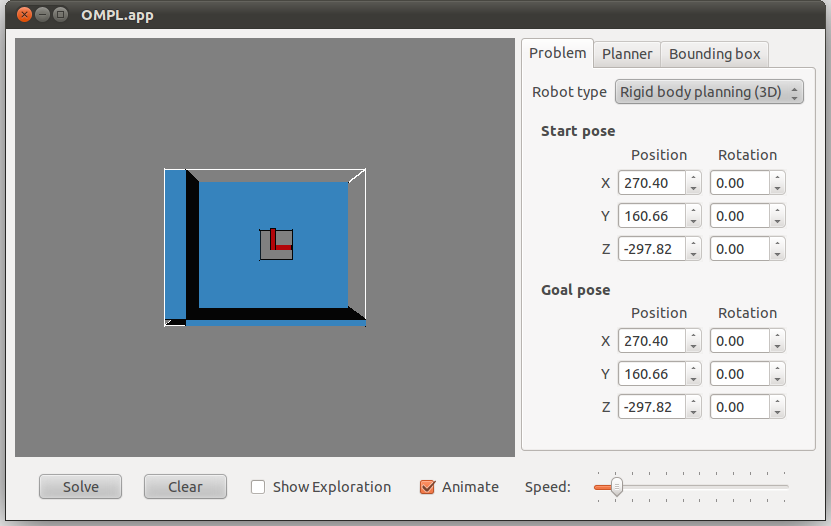
\includegraphics [width=3.5in]{omplapp_easy}
\caption {The ``easy'' environment loaded with the robot occupying the opening.}
\label {fig:omplapp:easy}
}
\end {figure}

Next the start and goal configurations must be chosen.  When a robot mesh is
first loaded, the start and goal poses are equivalent.  In the ``easy''
environment, the most interesting queries involve the robot maneuvering through
the opening in the wall.  One such configuration is $(270, 50, -200)$ and $(270,
50, -400)$, respectively.  Set the start and goal positions to these values and
click ``Solve'' to find a solution with the default planner.  The
default planner should not have too much trouble solving this query.  When a
solution is found the robot will become animated and travel along the computed
path.  If the planner fails to find a solution, repeat the solving process
until one is found.

The user can also switch between an animated robot and a view of the discrete
segments of the path by toggling the ``Animate'' check box.  Also, a
projection of the random samples can be seen by checking the ``Show
Exploration'' box.  In a bi-directional planner, the samples from each direction
will be shown as different colors.

\begin {figure}[h]
\centering
{
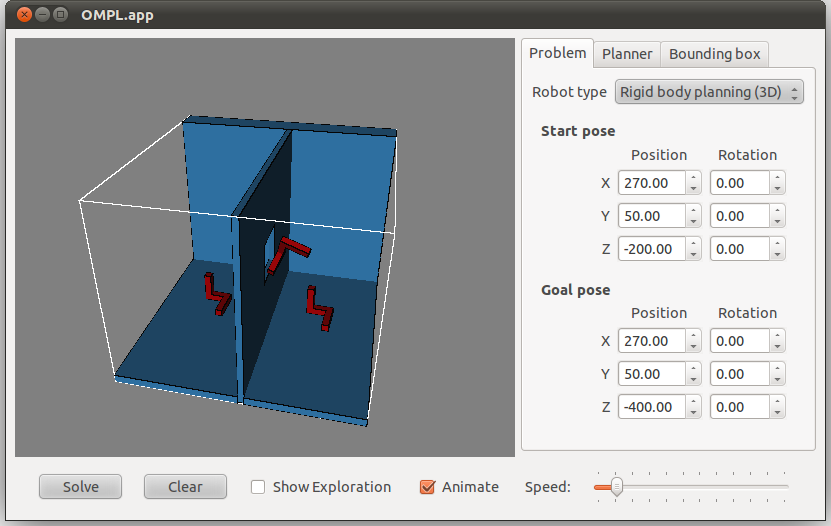
\includegraphics [width=3.5in]{omplapp_easy_sln}
\caption {The ``L'' shaped robot moving through the narrow passage.}
\label {fig:omplapp:easysolution}
}
\end {figure}

\subsection {Choosing a Planner}
Due to the wide variety in how sampling-based planners operate, selecting a
different planner may yield better results for a specific query.  Moreover,
the amount of time allotted to the planner can be customized.  In geometric
instances, the collision checking resolution that is employed by the local
planner can be changed to improve performance.  For instances that use motion
controls, the propagation step size for each control can be specified, as
well as the range of possible steps to apply the control.  In addition to these
general parameters, many of these methods have parameters that can be tuned
to further improve the time needed to solve a query and/or the quality of the
solution returned.  OMPL.app exposes these parameters, many of which are common
amongst the various planners, under the ``Planner'' tab.  The following defines
the most common parameters seen in geometric and control based planners in OMPL:

\begin{description}
\item[Range:] This parameter represents the maximum length of a motion
to be added in the tree of motions. It greatly influences the runtime of the
algorithm.

\item[Goal bias:] In the process of randomly selecting states in the state
space to attempt to go towards, the algorithm may in fact choose the actual goal
state with some probability. This probability is a real number between 0.0 and
1.0; it should not be too large, and usually lies around 0.05.

\item[Border fraction:] Planners such as {\tt KPIECE} use a discretization
of a projection of the state space to guide the exploration. This discretization
consists of a set of cells. The border fraction is the fraction of time spent
focusing the exploration on border cells (cells at the exploration ``frontier'').
This represents the minimum percentage used to select cells that are on the
border (minimum because if 95\% of cells are on the border, they will be
selected with 95\% chance, even if the border fraction is set to 0.9 (90\%)).

\item[Max.\ nearest neighbors:] The maximum number of nearest neighbors for
which a connection will be attempted when a new configuration sample is added.
\end{description}

Every effort is made to set the defaults for these settings to values that are
conducive in general planning environments.  However, depending on the
difficulty of the query, these settings may need to change to yield better
performance.  Consult the literature for the different planners to understand
how changing a specific parameter will change the behavior of a method in a
particular instance.

\subsection {Bounding the Environment}
By default, the robot is constrained to move inside a tight bounding box around
the environment, the start pose, and the goal pose. The bounding box is
visualized in OMPL.app as the white frame around the environment and robot.
These bounds apply to a reference point for the robot; the origin of the
coordinate frame that defines its pose. This means that parts of the robot can
stick outside the bounding box. It also means that if the reference point for
your robot is far away from the robot itself, you can get rather unintuitive
results. The reference point is whatever the origin is in the mesh; OMPL.app is
not using the geometric center of the mesh as the reference point.

\subsection {Saving and Replaying Solution Paths}
OMPL.app also has the ability to save the current solution path and reload that
path for viewing in the future.  Once a problem has been solved, the solution
found can be saved to a text file by selecting ``Save Path'' from the File menu.
A save dialog will be presented to select a directory and filename to save the
path to. Similarly, the path can be reloaded and replayed by selecting ``Load
path'' from the File menu.  The environment or robot mesh data is not saved in
this path file.  The same environment and robot must be reselected by the user
to replay the same path.

\section {OMPL.app vs.\ OMPL}
OMPL.app builds upon the motion planning functionality in OMPL by specifying
a geometric representation for the robot and its environment, and provides
a collision checking mechanism for the representation to the existing planners
in the library.  OMPL.app makes use of open-source collision checking
libraries \cite{Larsen:2000, Jia:2011}.  The core Open Motion Planning
Library does not explicitly represent the robot or the environment, and it is
up to the user to make this decision for their particular application.

OMPL has also been integrated with ROS. In ROS the robot and environment can
be represented with geometric meshes, but a model of the environment can also
be obtained as a point cloud from sensor data. ROS also provides a file
format for specifying articulated mechanisms that, when parsed, cause the
appropriate state space for planning to be created.


\chapter {Planning with OMPL}
\label {chp:ompl}

The Open Motion Planning Library provides an abstract representation for all
of the core concepts in motion planning, including the state space, control space,
state validity, sampling, goal representations, and planners.  This chapter
discusses OMPL and how its components relate to the ideas from the motion
planning literature.  The first section discusses the design considerations of
the library.  The second section maps the components of OMPL to their logical
equivalents in the motion planning literature.  The third elaborates on the
use of OMPL for solving motion planning queries using sampling-based techniques
composed from the objects described in Chapter \ref{chp:motionplanning}.  The
fourth section details the compilation of code written using OMPL, and the final
discusses OMPL's benchmarking capabilities.

There exists a wide variety of documentation, tutorials, and other examples
regarding the use of OMPL at {\tt ompl.kavrakilab.org}.  Specifically, the
website has extensive resources for installation, hands-on tutorials, as well
as the API documentation.  Additionally, a group exists at {\tt sourceforge.net}
called ``ompl-users'', which contains a forum for posting comments, questions,
and bug reports.

\section {Design Considerations}
\label{chp:design}
OMPL is flexible and applicable to a wide variety of robotic systems.  As a
consequence to this flexibility, the library does not explicitly represent the
geometry of the workspace or the robot operating in it.  This is deliberate
since there exists a vast amount of file formats, data structures and other
means of representation for robotic systems.  As a result, the user must select
a computational representation for the robot and provide an explicit state
validity/collision detection method.  There does not exist a default collision
checker in OMPL.  This allows the library to operate with relatively few
assumptions, allowing it to plan for a huge number of systems while remaining
compact and portable.

A conscious effort is also made to limit the number of external dependencies
necessary to compile and execute the code in OMPL.  The majority of the third
party code utilized in the library used comes from Boost \cite{Boost}, which
allows OMPL to function in most major operating systems.  Currently, OMPL is
supported on Linux and macOS.  Windows installation of the core OMPL
library is also possible by compiling from source.  Installation of OMPL.app on
Windows can also be done, but this is recommended only for experienced Windows
developers as the installation of the dependencies is challenging.

\section {OMPL Foundations}
Chapter \ref{chp:motionplanning} showed that many sampling-based motion planners
require a few similar components to solve a planning query: a sampler to compute
valid configurations of the robot, a state validity checker to quickly evaluate
a specific robot configuration, and a local planner to connect two samples along
a collision free path.  OMPL provides most of these components in similarly
named classes.  The following OMPL classes are analogous to ideas in traditional
sampling-based motion planners:

\paragraph {StateSampler} The StateSampler class implemented in OMPL
provides methods for uniform and Gaussian sampling in the most common state
space configurations.  Included in the library are methods for sampling
in Euclidean spaces, the space of 2D and 3D rotations, and any combination
thereof with the CompoundStateSampler.  The ValidStateSampler takes advantage
of the StateValidityChecker to find valid state space configurations.

\paragraph {NearestNeighbors} This is an abstract class that is utilized
to provide a common interface to the planners for the purpose of performing a
nearest neighbor search among samples in the state space.  The core library
has several types of nearest neighbor search strategies at its disposal,
including Geometric Near-neighbor Access Trees (GNATs)~\cite{Brin:1995}
and linear searches.
It is also possible to use an external data structure and supply the core library
with this implementation.

\paragraph {StateValidityChecker} The StateValidityChecker is tasked with
evaluating a single state to determine if the configuration collides with an
environment obstacle and respects the constraints of the robot.  A default
checker is \emph{not} provided by OMPL for reasons stated in Section
\ref{chp:design}.  Since this component is an integral part of sampling-based
motion planning it is necessary for the user to provide the planner a callback
to such a method to ensure that all configurations are feasible for the robot.

\paragraph {MotionValidator} The MotionValidator class (analogous to the local
planner) checks to see if the motion of the robot between two states is valid.
At a high level, the MotionValidator must be able to evaluate whether the motion
between two states is collision free and respects all the motion constraints of
the robot.  OMPL contains the DiscreteMotionValidator, which uses the
interpolated movements between two states (computed by the StateSpace) to
determine if a particular motion is valid. This is an approximate computation as only a finite number of states along the motion are checked for validity (using the StateValidityChecker).

\paragraph {OptimizationObjective} Certain motion planners can meet optimization 
objectives as well. These objectives can implement different cost functions.
The OptimizationObjective class provides an abstract interface to the relevant operations with costs that the planners need.
There are multiple default optimization objectives already implemented. For example, to minimize path length, a
PathLengthOptimizationObjective (derived from OptimizationObjective) can be used.

\paragraph {ProblemDefinition} A motion planning query is specified by the
ProblemDefinition object.  Instances of this class define a start state and goal
configuration for the robot, and the optimization objective to meet, if any. 
The goal can be a single configuration or a region surrounding a particular state.
Solutions to motion planning queries are also retrieved using this class.

\section {Solving a Query}
The previous set of objects are just a subset of the classes used in OMPL.
Figure \ref{fig:ompl:hierarchy} shows the hierarchy of the major components
of OMPL and how they are interrelated.

\begin {figure}[h]
\centering
{
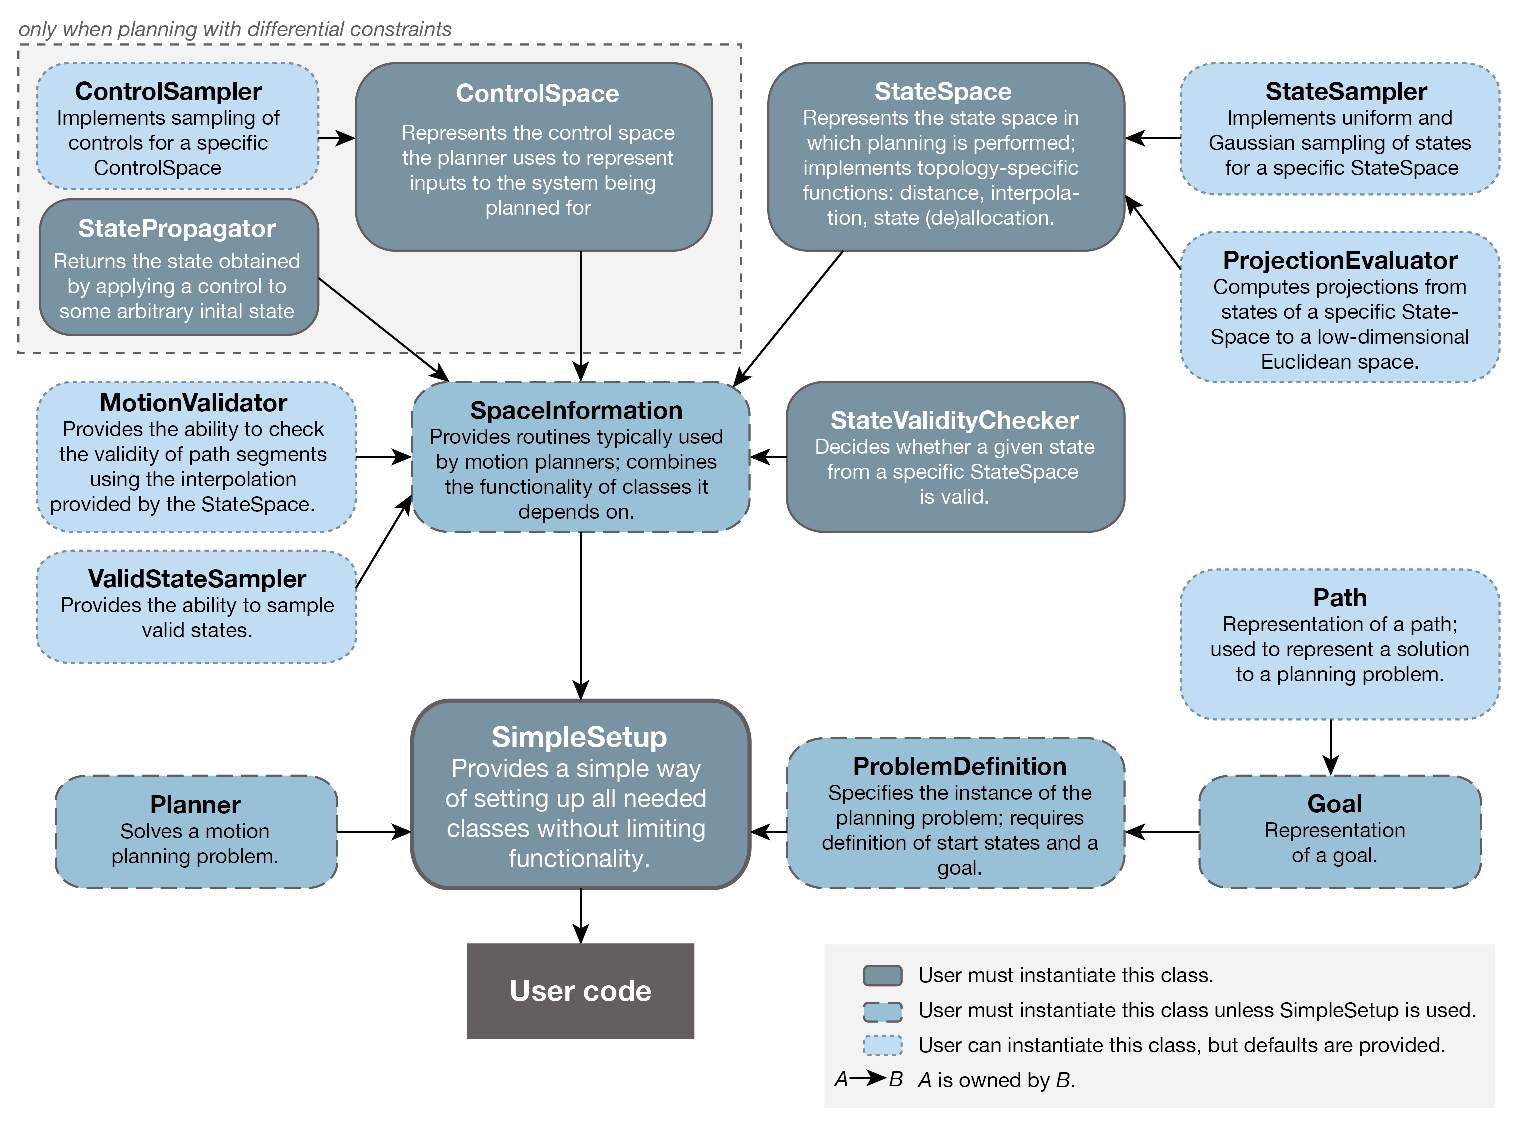
\includegraphics [width=.9\textwidth]{ompl_hierarchy}
\caption {The hierarchy of the high level components of OMPL.  Objects
highlighted in dark blue are required to be instantiated by the user.}
\label {fig:ompl:hierarchy}
}
\end {figure}

The object oriented nature of OMPL allows the user to inherit from currently
existing components or create brand new components to plan for a specific
system.  When solving a particular query, the user is not required to
instantiate all of the objects detailed in Figure \ref{fig:ompl:hierarchy}.
In fact, most of these objects have default implementations that are
sufficient for general planning.

\paragraph {Geometric Planning}
For geometric motion planning, the user must define and instantiate the state
space object for the robot, and provide a start and goal configuration in that
space to define the motion planning query.  Any planner defined in the
geometric namespace can then be employed to solve the motion planning query.
Some of these planners (as indicated by the planner specification) also follow 
optimization objectives.

\paragraph {Planning with Controls}
Like geometric planning, when planning with controls the user must define and
instantiate the state space for the robot, and provide a start and goal
configuration.  In addition, the user must define valid control inputs via
a ControlSpace object, and provide a method for computing how the system state
changes when applying valid controls using a StatePropagator instance.  The
user can use any planner in the control namespace to compute a solution.

\paragraph {SimpleSetup}
SimpleSetup provides a way to encapsulate the various objects necessary to
solve a geometric or control query in OMPL.  When using SimpleSetup, the user
only supplies the state space, start state, and goal state (and state propagator
for planning with controls). Specifically, SimpleSetup instantiates the
SpaceInformation, ProblemDefinition, and Goal objects.  Additionally,
SimpleSetup allows for the retrieval of all of these subcomponents for further
customization.  This means that SimpleSetup does not inhibit any native
functionality of OMPL, and ensures that all objects are properly created before
planning takes place.  Moreover, SimpleSetup exposes fundamental function
calls for ease of use.  For example, the function ``solve'' from the Planner
class is available in SimpleSetup, and it is not necessary for the user to
extract the Planner from the SimpleSetup instance to do so.

\section {Compiling Code with OMPL}
Once a new planner, sampler, collision checker, or other motion planning
component has been developed, it is simple to integrate with OMPL for testing.
There are two methods for compiling code with OMPL.  If the base library is
modified (e.g., a new planner is added to  {\tt ompl/geometric/planners}),
simply re-run \emph{cmake} to reconfigure the makefiles for that particular
component of the code.  If the new code does not exist in a directory known to
\emph{cmake}, {\tt ompl/src/ompl/CMakeLists.txt} will need to be updated to
search in the extra directory.

If OMPL has been installed, new code can be compiled independently from OMPL.
The core OMPL library can be linked into the final binaries using the
traditional linking step.  For example, if compiling with GCC, simply link the
code with ({\tt -lompl}), and direct the compiler to search the install
directory for the library.  A similar linking procedure can be employed
with other compilers.

\section {Benchmarking}
The ability to compare two or more planners has never been easier than with
OMPL.  OMPL provides a Benchmark class that attempts a specific query a given
number of times, and allows the user to try any number of planners.
Additionally, the Benchmark instance can be configured to fail an attempt after
a specific amount of time or when the planner exhausts a given amount of memory.
If multiple instances of the same type of planner are to be benchmarked (e.g., with 
different sets of settings), changing the planner name is a good idea 
(Planner::setName() function), so that the results can be distinguished.

When the benchmarking has finished, the Benchmark instance will write a log
file to the current working directory containing information regarding every
planning attempt.  OMPL is packaged with a Python script to parse this log file
and create an SQL database with the planning information.  The Python script can
also query this database and generate a series of plots using matplotlib, like
those in Figure \ref {fig:benchmark:plot}.

\begin {figure}
\centering
{
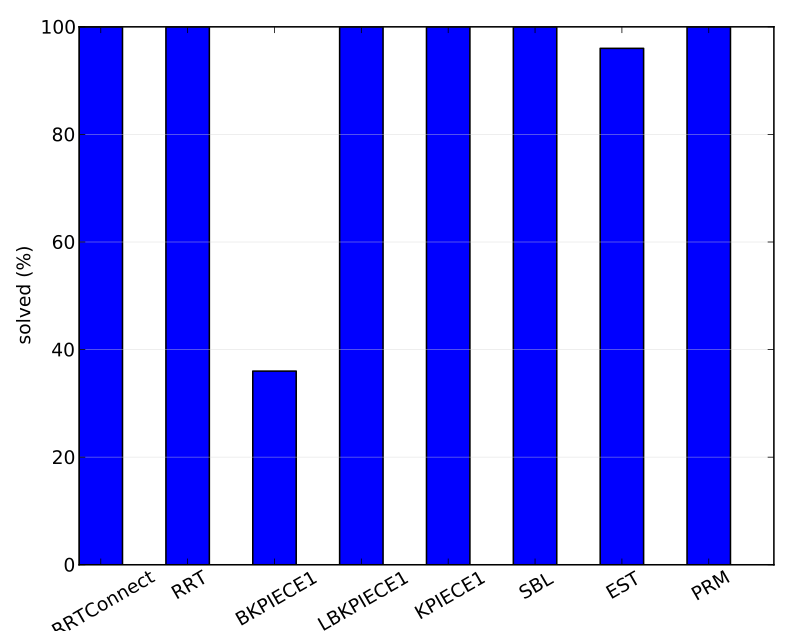
\includegraphics [width=3.75in]{twistycool_solved}\\ \vspace {0.25in}
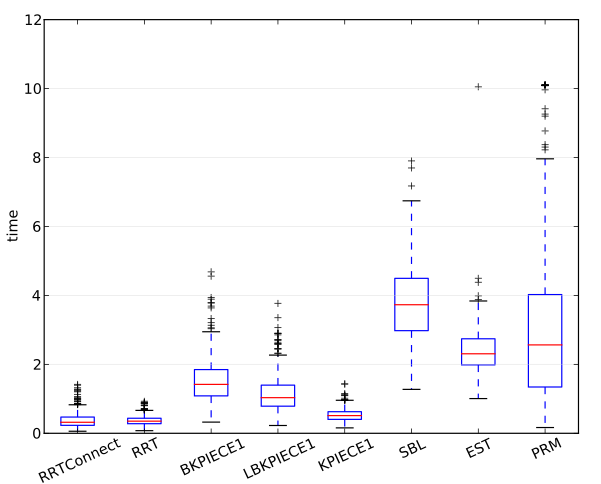
\includegraphics [width=3.75in]{cubicles_time}
\caption {Example benchmarking plots. (top) The percentage of instances solved by various
planners during one benchmark run. (bottom) A box plot showing the amount of time needed
for various planners to solve a planning instance}
\label {fig:benchmark:plot}
}
\end {figure}


\chapter{Advanced Topics in OMPL}

This chapter explains some of the more advanced features of OMPL.  This section
is not meant to explain all of the expert level concepts, but to give the user
an idea about some commonly used optional features of the library and how they
can be included in the code.  API documentation is updated regularly at
{\tt ompl.kavrakilab.org}, and includes the following concepts, among others.

\section {State Space Construction}
OMPL provides implementations for several common states spaces, including
${\mathbb R}^n$ for euclidean spaces and SO(2) and SO(3) for the space of
rotations in 2D and 3D respectively.  Many systems operate in spaces
that are combinations of ${\mathbb R}^n$ and orientations.  For example, the
classic ``piano mover's'' problem operates in SE(3), which is a combination
of ${\mathbb R}^3$ and SO(3).  OMPL contains an implementation of the SE(2) and
SE(3) state spaces for such instances.

In complex systems, like highly articulated robot arms, it is infeasible to
enumerate all possible state spaces.  However, the state spaces in many of these
systems can be decomposed into smaller spaces (like the SE(3) example).  To
accommodate this, OMPL allows for the construction of such spaces through the
CompoundStateSpace class, which allows state spaces to be formed from a
combination of their subcomponents.  The existing state spaces all provide
operator overloads for the `+' and `$-$', allowing readable and intuitive code to
be written when constructing such spaces.

\section {Planner Customization}
In the motion planning literature, there exist many variants of the classical
planning algorithms that change only one component of the planning algorithm
in order to achieve benefits in certain instances.  Many of the planners that
come bundled with OMPL are highly customizable, and in some cases it isn't
necessary to derive a new planner from the existing code base to recreate one of
these variations or test a new idea or algorithm.

An easy example is the nearest neighbor search performed in nearly all of the
planners to find the closest existing state to a newly generated random sample.
There are many algorithms to perform this search---both exact and
approximate---and evaluating the best approach for one particular system can become time
consuming.  The {\tt PRM} and {\tt RRT} planners (among others) both provide a
hook to replace the default nearest neighbor search with a user supplied
object that derives from the abstract NearestNeighbor class.  This allows users
to develop compact and portable components for differing nearest neighbor
schemes and test them without creating unnecessary planner objects that are
simply one-off from one another.  Similar possibilities exist not only with
nearest neighbor searching, but also in other planning components, like state
sampling and connection strategies.

\section {Python Bindings}
Users of OMPL are not bound to C++.  Most of the API is exposed through a set
of Python bindings from which users can create Python scripts to solve motion
planning queries.  These bindings are compiled separately from the OMPL core
library, and require Py++ and Boost.Python for correct operation.  Ensure that
these dependencies exist before installing OMPL to create the bindings. The
Python bindings are still considered an experimental feature and all API
documentation is for the C++ API (although we have tried to keep the python API
as similar as possible). The easiest way to get started with the python bindings
is by looking at a few of the demo programs.

The bindings are separated by ompl namespaces into python modules contained
within one parent {\tt ompl} module.  For example, to use a geometric motion
planner from OMPL, the {\tt base} and {\tt geometric} modules must be imported:
\\
{\tt from ompl import base\\
from ompl import geometric}

There are some subtle and some not-so-subtle differences between the C++ and
Python APIs due to the differences between the two programming languages.  A
user checking the OMPL C++ API must note the following discrepancies when
writing a program in Python:

\begin {itemize}
\item An STL vector of int's is of type vectorInt in Python (analogously for
other types).
\item The C++ class State has been renamed AbstractState, while the C++ class
ScopedState<> is called State in Python.
\item The C++ class ScopedState<RealVectorStateSpace> is called RealVectorState.
The ScopedState's for the other pre-defined state spaces have been renamed
analogously.
\item The C++ class RealVectorStateSpace::StateType has been renamed to
RealVectorStateInternal (analogously for the other state space types), to
emphasize that a user should really be using RealVectorState.
\item Use the ``()'' operator on a ScopedState in Python to retrieve a reference
to a C++ State.
\item The print method (for classes that have one) is mapped to the special
python method \_\_str\_\_, so a C++ call like {\tt foo.print(std::cout)} becomes
{\tt print foo} in python. Similarly, a C++ call like
{\tt foo.printSettings(std::cout)} becomes {\tt print foo.settings()} in python.
\item The signature of the state validity checker is changed. In python the
state validity checker has the following form:
\begin {verbatim}
def isStateValid(spaceInformation, state):
    return spaceInformation.satiesfiesBounds(state)
\end {verbatim}

\end {itemize}



\bibliographystyle {unsrt}
\bibliography {Primer}

\end {document}

